\section{Definition of an Event Tree}
\label{sec:event_tree_definition}

Event trees unravel how a single \emph{initiating event} (\(I\)) can branch into multiple possible \emph{end-states} (\(X\)) through a sequence of \emph{functional} (or conditional) events. Each branch captures the success or failure of an important \emph{functional event} (e.g.\ a safety barrier or operator intervention). By following all possible paths, one can systematically account for each final outcome \(X_j\). Figure~\ref{fig:event_tree_example} provides a schematic view of this process for an initiating event \(I\) and two subsequent functional events, \(F_1\) and \(F_2\). Each terminal node (leaf) corresponds to a distinct end-state, denoted \(X_1, X_2, \ldots, X_n\). Though this illustration is intentionally simple, more complex systems may include numerous functional events, each branching into further outcomes.

\begin{figure}[ht!]
\centering
\begin{tikzpicture}
\tikzset{grow'=right,level distance=48pt}
\tikzset{execute at begin node=\strut}
\tikzset{every tree node/.style={anchor=base west}}
\tikzset{
    edge from parent/.append style={very thick},
    edge from parent/.style={
        draw,
        edge from parent path={
            (\tikzparentnode.east) -| ($(\tikzparentnode.east)!0.5!(\tikzchildnode.west)$) |- (\tikzchildnode.west)
        },
    },
    every node/.style={anchor=center,font=\small\bfseries, text centered, inner sep=0pt},
    every level 0 node/.style={circle, font=\small\bfseries, draw, fill=blue!30, inner sep=0pt},
    every internal node/.style={font=\small, inner sep=4pt},
    every leaf node/.style={rectangle, draw, fill=blue!30, minimum width=2.5cm, text centered},
    frontier/.style={distance from root=400pt},
}
\Tree [.\(I\)
    [.\(F_1^{\text{succ}}\)
        [.\(F_2^{\text{succ}}\)
            [.\(X_1\) ]
        ]
        [.\(F_2^{\text{fail}}\)
            [.\(X_2\) ]
        ]
    ]
    [.\(F_1^{\text{fail}}\)
        [.\(X_3\) ]
    ]
]
\end{tikzpicture}
\caption{Illustrative event tree with an initiating event \(I\), two functional events \(F_1\) and \(F_2\), and three end-states \(X_1, X_2, X_3\).}
\label{fig:event_tree_example}
\end{figure}

At the highest conceptual level, an event tree is a collection of conditional outcomes. Let \(n\) be a positive integer, and let \(j\) range over some index set of end-states~\(J\). Then define
\begin{equation}
\label{eq:event_tree_gamma}
    \Gamma
    \;=\;
    \Bigl\{
        \langle
            I,\,
            F_1,\,
            F_2,\,
            \dots,\,
            F_n,\,
            X_j
        \rangle
        :\,
        j \in J
    \Bigr\},
\end{equation}
where:
\begin{itemize}
    \item \(I\) is the \textbf{initiating event}. In a nuclear system, this could be an abnormal occurrence such as a coolant pump trip or an unplanned reactivity insertion.
    \item \(F_k\) (\(k=1,\ldots,n\)) denotes the \(k\)th \textbf{functional (conditional) event}, which may succeed (\(F_k^{\text{succ}}\)) or fail (\(F_k^{\text{fail}}\)). Typically, each \(F_k\) depends on the outcomes \(F_1,\ldots,F_{k-1}\).
    \item \(X_j\) is an \textbf{end-state}, describing the final outcome along a particular branch. End-states might indicate safe shutdown, core damage, or a radiological release.
\end{itemize}
Each tuple \(\langle I, F_1, \dots, F_n, X_j\rangle\) in \(\Gamma\) encapsulates a distinct scenario pathway. In the broader context of the risk triplet, such a pathway corresponds to \(S_i\), the possibility of something going wrong, while the associated probability and consequences map directly to \(L_i\) and \(X_i\).

\subsection{Probabilistic Representation}

Because risk analysis requires knowing how likely each branch in the tree is, event trees rely heavily on \emph{conditional probabilities}. Let
\[
    p(I)
    \;\equiv\;
    \Pr(I)
\]
be the probability (or frequency) of the initiating event. For each functional event \(F_k\), define
\[
    p\bigl(F_k^{\text{succ}}\mid I,\, F_1,\,\dots,\,F_{k-1}\bigr)
    \quad\text{and}\quad
    p\bigl(F_k^{\text{fail}}\mid I,\, F_1,\,\dots,\,F_{k-1}\bigr),
\]
which describe the likelihood of success or failure given all prior outcomes.

An \emph{end-state} \(X_j\) arises from a particular chain of successes/failures:
\[
    \bigl(I,\,F_1^{\alpha_1},\,F_2^{\alpha_2},\,\ldots,\,F_n^{\alpha_n}\bigr)
    \;\longrightarrow\; 
    X_j,
\]
where each \(\alpha_k \in \{\text{succ},\,\text{fail}\}\). The probability of reaching \(X_j\) is the product of:
\begin{enumerate}
    \item The initiating event probability \(p(I)\).
    \item The conditional probabilities of each functional event's success or failure.
\end{enumerate}
Formally, if \(\omega_j\) denotes the entire branch leading to end-state \(X_j\), then
\begin{align}
\label{eq:event_tree_branch_probability}
    p(\omega_j)
    \;=\;
    p(I)
    \times
    \prod_{k=1}^{n}\,
    p\!\bigl(F_k^{\alpha_k}\mid 
             I,\,
             F_1^{\alpha_1},\ldots,
             F_{k-1}^{\alpha_{k-1}}\bigr).
\end{align}
The union of all such branches spans the full sample space of scenario outcomes generated by \(I\) and the subordinate functional events. Next, we show that every branch of an event tree can be represented by a product (logical AND) of the relevant Boolean variables for the initiating event and each functional event’s success/failure.  Collecting all branches via logical OR yields a disjunction of these products, precisely matching the standard structure of a Boolean expression in disjunctive normal form (DNF).

\subsection{Event Tree Structures as Sum-Product Networks}
Consider a specific branch \(\omega_j\) leading to the end-state \(X_j\).  By definition, \(\omega_j\) occurs if and only if:
\begin{enumerate}
    \item The initiating event \(I\) happens: \(i=1\).
    \item For each functional event \(F_k\), the branch specifies a particular outcome (success or failure).  Suppose \(\omega_j\) includes successes for some subset of indices \(\alpha\subseteq \{1,\ldots,n\}\) and failures for the complementary indices.  We can write this as:
    \[
        \bigwedge_{k\in \alpha}  \bigl(f_{k}^{\text{succ}} = 1\bigr)
        \quad\wedge\quad
        \bigwedge_{k\notin \alpha} \bigl(f_{k}^{\text{fail}} = 1\bigr).
    \]
\end{enumerate}
Hence, the branch event \(\omega_j\) is logically equivalent to a single \emph{product term}:
\begin{equation}
\label{eq:branch_conjunction}
    \omega_j \;\equiv\; 
    \bigl(i=1\bigr)
    \;\wedge\;
    \bigwedge_{k\in \alpha} \bigl(f_k^{\text{succ}}=1\bigr)
    \;\wedge\;
    \bigwedge_{k\notin \alpha} \bigl(f_k^{\text{fail}}=1\bigr).
\end{equation}
In standard Boolean notation, each literal (e.g., \(f_k^{\text{succ}}\)) is a variable that can be 0 or 1, and the branch is the \(\land\) (AND) of those variables. An event tree describing all possible outcomes from \(I\) and the subsequent functional events can be viewed as the union (logical OR) of its disjoint branches:
\[
    \Omega \;=\; \omega_1 \;\cup\; \omega_2 \;\cup\;\cdots \;\cup\; \omega_m.
\]
In Boolean terms, this is the \(\lor\) (OR) of the product terms corresponding to each branch:
\begin{equation}
\label{eq:event_tree_disjunction}
    \Omega
    \;\equiv\;
    \omega_1
    \;\lor\;
    \omega_2
    \;\lor\;\cdots\lor\;
    \omega_m.
\end{equation}
Substituting each branch’s conjunction form (as in Eq.~\eqref{eq:branch_conjunction}) into Eq.~\eqref{eq:event_tree_disjunction} yields:
\[
    \Omega 
    \;\;=\;\;
    \Bigl[
        i \;\wedge\; \prod_{k\in \alpha_1} f_k^{\text{succ}} \;\wedge\; \prod_{k\notin \alpha_1} f_k^{\text{fail}}
    \Bigr]
    \;\;\lor\;\;
    \Bigl[
        i \;\wedge\; \prod_{k\in \alpha_2} f_k^{\text{succ}} \;\wedge\; \prod_{k\notin \alpha_2} f_k^{\text{fail}}
    \Bigr]
    \;\;\lor\;\;
    \cdots
\]
where each \(\alpha_r\) is the set of functional events that succeed along branch \(r\).

A standard DNF (sum-of-products) expression in Boolean algebra is
\[
    \bigl(\text{literal}_1 \;\wedge\;\text{literal}_2 \;\wedge\;\cdots\bigr)
    \;\;\lor\;\;
    \bigl(\text{literal}_{1}' \;\wedge\;\text{literal}_{2}' \;\wedge\;\cdots\bigr)
    \;\;\lor\;\;\cdots
\]
Each term in the sum (OR) is a logical AND of literals (variables or their negations). Comparing with Eq.~\eqref{eq:event_tree_disjunction}, we see that an event tree is exactly a disjunction of terms, each term being a conjunction of the initiating event \(i\) (set to 1) and the success/failure indicators for each \(F_k\). Since any negation can be encoded by stating whether \(F_k\) is \(\text{succ}\) (\(f_k^{\text{succ}}=1\)) or \(\text{fail}\) (\(f_k^{\text{fail}}=1\)), the entire event tree \(\Omega\) is in DNF:
\[
    \Omega \;=\; 
    \bigvee_{j=1}^m
    \Bigl[
        \;\bigwedge_{\ell\in \Lambda_j}
        (\text{appropriate literal})
    \Bigr].
\]

\subsection{Expressivity and Tractability of Event Trees}
\label{sec:tractability_event_trees}

Within \(\operatorname{SP}\!-\)networks (sum-product networks), a sum gate provides a weighted sum of child distributions, whereas a product gate factorizes them.  An event tree can be cast as an \(\operatorname{SP}\!-\)network by feeding each branch’s literal probabilities into product gates (one per branch), then summing over all branches with a sum gate.  Once constructed, evaluating the resulting \(\operatorname{SP}\!-\)network at a specific configuration \(\mathbf{x}\) or marginalizing out some of the variables is linear in the size of that network.  Nevertheless, the tractability of event trees (and their circuit representations) heavily depends on their size and structure.  We summarize several key considerations below:

\begin{enumerate}
    \item \emph{DNF size grows exponentially.}
    
    Suppose an event tree includes \(n\) functional events, each of which can succeed or fail.  In the worst case, enumerating \emph{all} possible outcome branches (i.e.\ each success/failure pattern) yields up to \(2^n\) conjunction terms.  Hence, the disjunctive normal form (DNF) representation can become exponentially large.  Computing or marginalizing probabilities over such a large DNF may become prohibitively expensive if \(n\) is large enough.

    \item \emph{Evaluation linear in network size.}
    
    Even though the DNF itself may blow up exponentially, once the event tree is translated into an \(\operatorname{SP}\!-\)network, key inference tasks (such as evaluating it at a configuration or marginalizing over certain variables) proceed in time linear in the \emph{compiled network size}.  That said, if the underlying network has already reached exponential size in the number of events, the linear-time evaluation does not necessarily improve the overall worst-case complexity.
    
    \item \emph{Approximations abound.}
    
    In practice, analysts often employ approximations to keep event trees tractable.  One possibility is \emph{decomposability}, a core principle behind tractable probabilistic circuits whereby each product gate operates on disjoint sets of variables.  If the system decomposes (e.g.\ different safety barriers protect disjoint sets of equipment), one can evaluate probabilities without enumerating all branches.  Another common approximation is to prune paths with very low probabilities or ignore paths that only negligiblly contribute to the overall risk.
\end{enumerate}

Fully enumerated event trees, regardless of being interpretable as DNF/SP networks, trade tractability for expressivity. The intuitive branching structure and conditional probability assignments make event trees easy to interpret. PRA analysts can read off and reason about the high-level scenario decomposition, incorporate domain knowledge, and analyze each branch explicitly.  If the number of critical functional events is moderate, enumerating all branches remains tractable. As the depth and breadth of the tree grow, any brute-force probability computation over such a large DNF/SOP circuit is equally exponential in the worst case. Even though \(\operatorname{SP}\!-\)networks offer efficient linear-time evaluation with respect to the circuit size, the underlying circuit itself may have size exponential in \(n\).